\section{Durchführung}
\label{sec:Durchführung}
\subsection{Justage}
Für die Durchführung des Versuches ist zunächst eine Justage der Apparatur nötig. Bei den verschieden Scans beträgt die Messdauer jeweils $t=\SI{1}{\second}$. Als erstes wird ein Detektorscan durchgeführt und das Maximum dieses Scans wird als Nullpunkt des Detektors genommen. Dieser Scan wird um den Nullpunkt durchgeführt von $\SI{-0.5}{\degree}$ bis $\SI{0.5}{\degree}$. Mithilfe eines Z-Scans wird die Probe so justiert, dass sie sich genau an der Position in Z-Richtung befindet an der die maximale Intensität $I_\mathrm{max}$ halbiert ist.
\begin{figure}[h!]
  \centering
  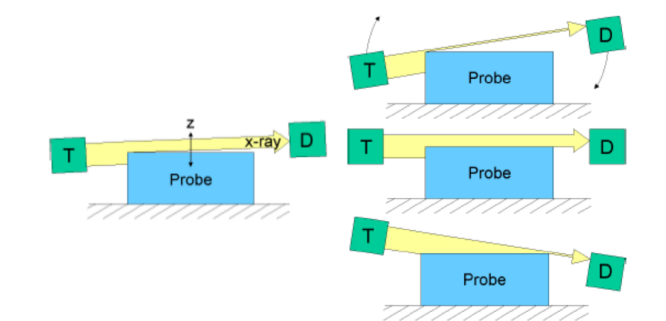
\includegraphics[scale=0.6]{fig/zscan.png}
  \caption{Schematische Darstellung des Z-Scans (links) und des Rockingscan (rechts). \cite[5]{Anleitung4}}
  \label{fig:zscanbei}
\end{figure}
\FloatBarrier
\noindent Mit einem X-Scan wird nun die Position in X-Richtung justiert.
Daraufhin wird ein Rockingscan durchgeführt, wobei der Detektor und die Röhre um die Probe gedreht werden. Als Ergebnis sollte ein gleichschenkliges Dreieck herauskommen. Falls dies nicht der Fall sein sollte, muss nachjustiert werden.
\begin{figure}[h!]
  \centering
  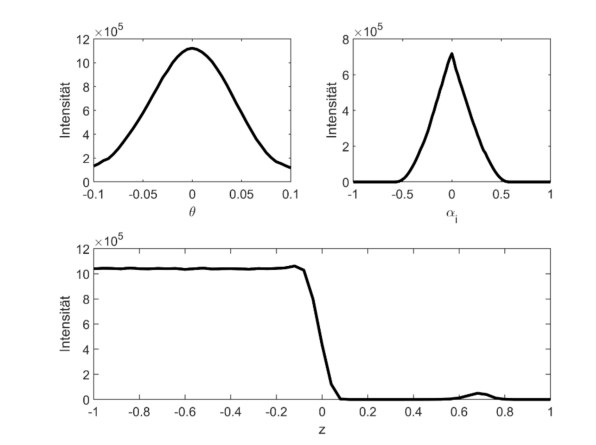
\includegraphics[scale=0.7]{fig/beispiel.png}
  \caption{Beispielplots von Detektorscan (oben links), Rockingscan (oben rechts) und Z-Scan (unten). \cite[6]{Anleitung4}}
  \label{fig:beispiele}
\end{figure}
\FloatBarrier
\noindent Durch die Ausrichtung im Rockingscan ist die Z-Position der Probe nicht mehr exakt, sodass ein weiterer Z-Scan durchgeführt wird. Für die Feinjustierung wird ein weiterer Rockingscan durchgeführt, dieser weicht vom ersten ab, da er unter einem Winkel von $2\theta=\SI{0.3}{\degree}$ durchgeführt wird. Es sollte ein deutlicher Reflex zu sehen sein.  Das Maximum der Kurve wird im Programm im Feld "Enter theorical Positon" auf $\SI{0.15}{\degree}$ gesetzt. Abschließend wird ein dritter Z-Scan durchgeführt, allerdings sind hier bei Detektor und Röhre jeweils um $\SI{0.15}{\degree}$ geneigt. Dies ist in Abbildung (\ref{fig:zscan015}) dargestellt.
\begin{figure}[h!]
  \centering
  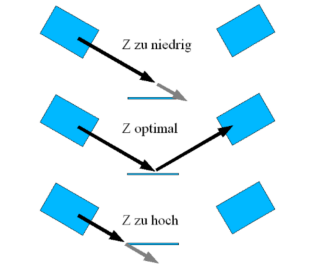
\includegraphics[scale=0.7]{fig/zscan015.png}
  \caption{Z-Scan mit geneigter Röhre und Detektor \cite[7]{Anleitung4}}
  \label{fig:zscan015}
\end{figure}
\FloatBarrier
\noindent Damit ist die Justage der Messapparatur abgeschlossen.
\subsection{Messung}
Nachdem die Justierung abgeschlossen ist, findet die eigentliche Messung der Probe statt. Dafür wird der "Omega/2Theta-Scan" verwendet. Der Scannbereich liegt dabei zwischen $\SI{0}{\degree}$ bis $\SI{2.5}{\degree}$ und die Schrittweite beträgt $\SI{0.005}{\degree}$ bei einer Messdauer von $t=\SI{5}{\second}$. Zusätzlich wird ein  "Diffuse Scan" durchgeführt, wo der Detektor um $\SI{0.1}{\degree}$ zur Röntgenröhre geneigt ist. Die sonstigen Einstellungen bleiben dabei gleich. \\
Abschließend werden die aufgenommenen Messdaten mit FileExchanger von einer .raw-Datei in eine .UXD-Datei umgewandelt und können ausgewertet werden.
